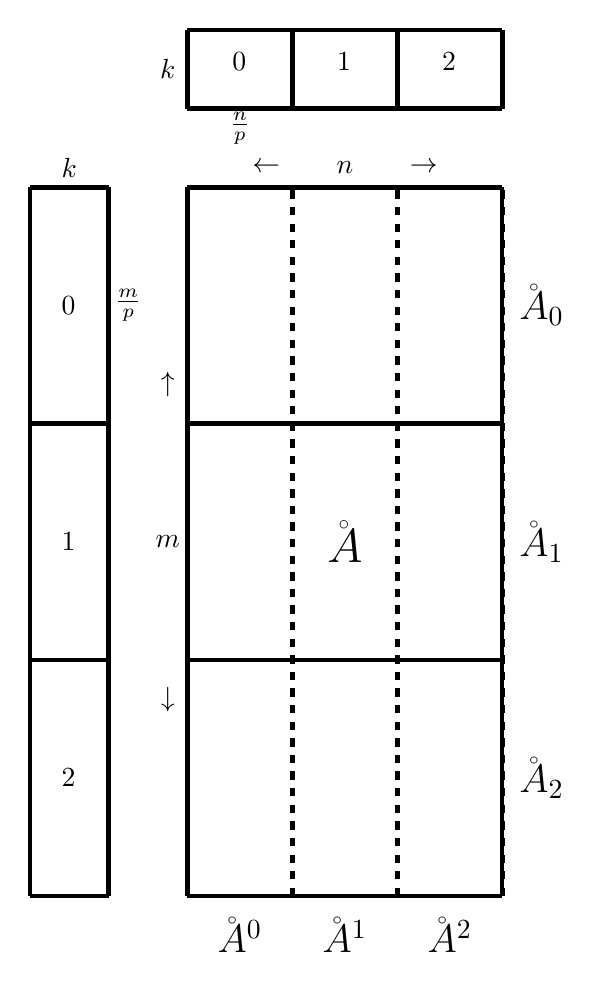
\begin{tikzpicture}

%% draw matrix distributions with scaled grids
% A
\draw[xscale=4/3,yscale=9,ultra thick, dashed] (0,0) grid (3,1);
\draw[xscale=4,yscale=3,ultra thick] (0,0) grid (1,3);
% W
%\draw[yscale=3/2] (-2,0) grid (-1,6);
\draw[yscale=3,ultra thick] (-2,0) grid (-1,3);
% H
%\draw[xscale=2/3] (0,10) grid (6,11);
\draw[xscale=4/3,ultra thick] (0,10) grid (3,11);

%% add (sub)matrix names 
% A
\node[draw=none] at (2,4.5) {\LARGE $\AA$};
\node[draw=none] at (4.5,7.5) {\Large $\AA_0$};
\node[draw=none] at (4.5,4.5) {\Large $\AA_1$};
\node[draw=none] at (4.5,1.5) {\Large $\AA_2$};
\node[draw=none] at (2/3,-0.5) {\Large $\AA^0$};
\node[draw=none] at (2,-0.5) {\Large $\AA^1$};
\node[draw=none] at (10/3,-0.5) {\Large $\AA^2$};
% W
\node[draw=none] at (-1.5,-0.5) {\LARGE $\WW$};
\node[draw=none] at (-1.5,7.5) {\Large $\WW_0$};
\node[draw=none] at (-1.5,4.5) {\Large $\WW_1$};
\node[draw=none] at (-1.5,1.5) {\Large $\WW_2$};
% H
\node[draw=none] at (-1,10.5) {\LARGE $\HH$};
\node[draw=none] at (2/3,10.5) {\Large $\HH^0$};
\node[draw=none] at (2,10.5) {\Large $\HH^1$};
\node[draw=none] at (10/3,10.5) {\Large $\HH^2$};

% label vertical dimensions
\node[draw=none] at (-0.25,10.5) {$k$};
\node[draw=none] at (-0.25,4.5) {$m$};
\node[draw=none] at (-0.25,6.5) {$\uparrow$};
\node[draw=none] at (-0.25,2.5) {$\downarrow$};
\node[draw=none] at (-0.75,7.5) {$\frac{m}{p}$};
% label horizontal dimensions
\node[draw=none] at (-1.5,9.25) {$k$};
\node[draw=none] at (2,9.25) {$n$};
\node[draw=none] at (1,9.25) {$\leftarrow$};
\node[draw=none] at (3,9.25) {$\rightarrow$};
\node[draw=none] at (2/3,9.75) {$\frac{n}{p}$};

\end{tikzpicture}